\documentclass[10pt,showpacs,preprintnumbers,footinbib,amsmath,amssymb,aps,prl,twocolumn,groupedaddress,superscriptaddress,showkeys]{revtex4-1}
\usepackage{graphicx}
\usepackage{dcolumn}
\usepackage{bm}
\usepackage[colorlinks=true,urlcolor=blue,citecolor=blue]{hyperref}
\usepackage{color}
\begin{document}
\title{FYS3150 Project 1}
\author{E.~Ludvigsen}
\noaffiliation
%\affiliation{Department of Something, University of Somewhere, Outer Space}
\begin{abstract}
Numerical solutions of the one-dimensional Poisson equation, by rewriting into a set of linear equations. 
\end{abstract}
\maketitle


\section{Introduction}


\section{Theory, algorithms and methods}


\section{Results and discussions}


\begin{figure}[hbtp]
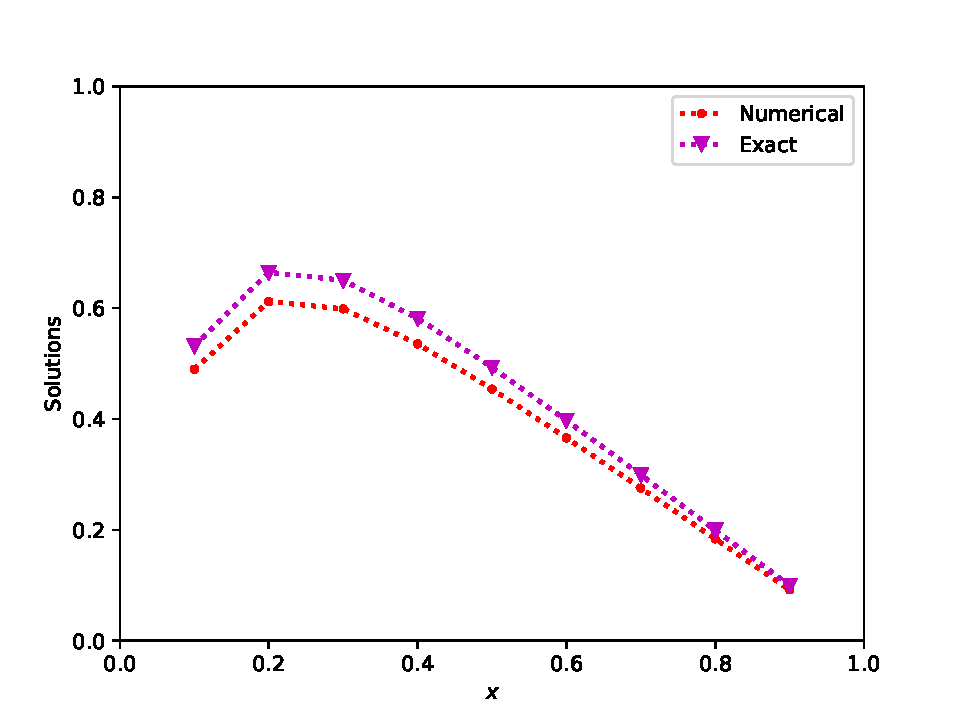
\includegraphics[scale=0.4]{../Output/TridiagonalSimple_out1.pdf}
\caption{Exact and numerical solutions for $n=10$ mesh points, simple forwards and backwards substitution.}
\label{fig:TridiagonalSimple_out1}
\end{figure}

\begin{figure}[hbtp]
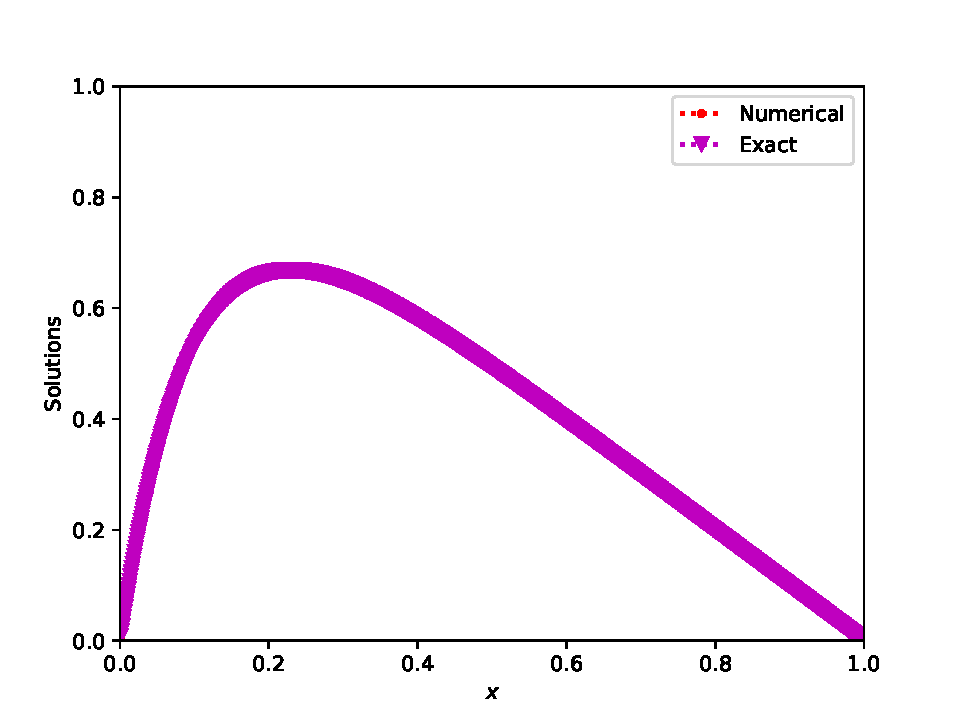
\includegraphics[scale=0.4]{../Output/TridiagonalSimple_out3.pdf}
\caption{Exact and numerical solutions for $n=1000$ mesh points, simple forwards and backwards substitution.}
\label{fig:TridiagonalSimple_out3}
\end{figure}

\begin{figure}[hbtp]
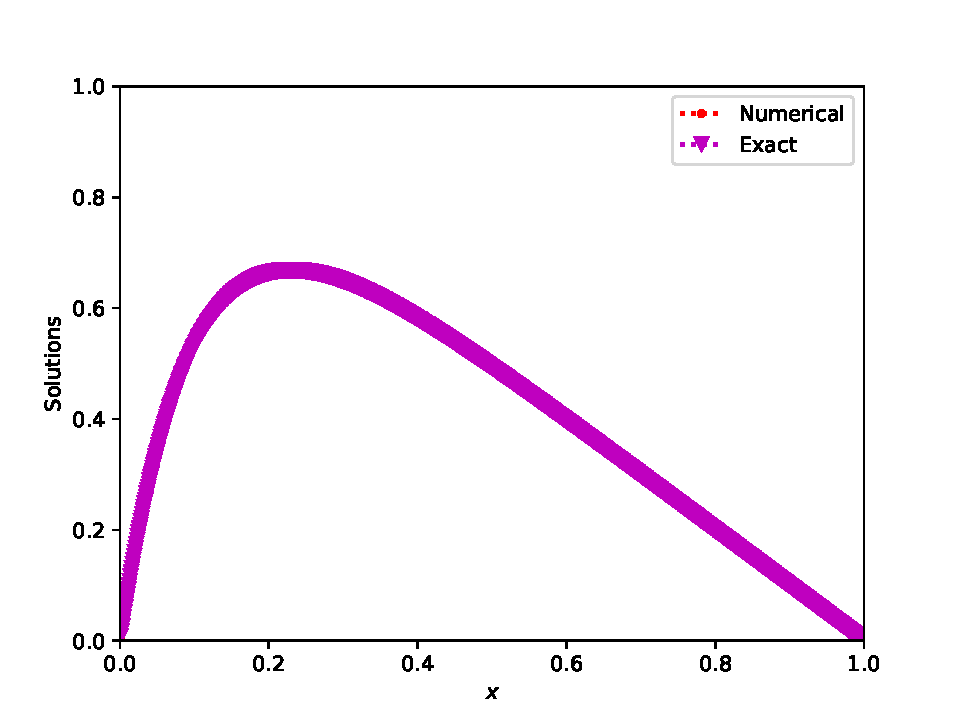
\includegraphics[scale=0.4]{../Output/TridiagonalArma_out3.pdf}
\caption{Exact and numerical solutions for $n=1000$ mesh points, Armadillo solver.}
\label{fig:TridiagonalArma_out3}
\end{figure}


\section{Conclusions}


\begin{thebibliography}{99}
%\bibitem{miller2006} G.~A.~Miller, A.~K.~Opper, and E.~J.~Stephenson, Annu.~Rev.~Nucl.~Sci.~{\bf 56}, 253 (2006).
\end{thebibliography}

\end{document}